\documentclass[ExampleMasters.tex]{subfiles}
\begin{document}
\chapter{Optimisation Results}

\section{Introduction}
As set out in the abstract, the generic vehicle model described in the Chapter 4 is used in consonance with the genetic algorithm described in Chapter 2 to derive optimal vehicle propulsion configurations for years 2015, 2020, 2025 and 2030, the objective function optimised being the vehicle productivity over the lifetime of the first owner's holding.\\

In this chapter, the results of the optimisation shall be presented in four different sub-sections. The first contains a brief listing of the results derived from successive runs of the genetic algorithm lasting 100 generations each. The following subsections are an analysis of the results in different headings.

\section{Overview of the results}
Optimal axle propulsion configurations are derived for the years specified above. The following tables list the results for varying gross combination weights of 50t, 60t, 70t and 80t for each of the four years in succession.

\begin{table}[ht]
\caption{Optimal combination configurations - Year 2015}
\centering
\begin{tabular}{c c c c c c}
\hline\hline
GCW & \multicolumn{4}{c}{Optimal configuration} & Vehicle Productivity \\ \cline{2-5}
(t) & Tractor & Semi-trailer & Dolly & Semi-trailer & (\euro/\euro)\\ 
\hline
50 & 010\textbackslash000\textbackslash011 &
	 001\textbackslash001\textbackslash000 & 100\textbackslash001\textbackslash00 &
	 100\textbackslash001\textbackslash000 & 0.960028 \\
60 & 100\textbackslash000\textbackslash011 &
	 001\textbackslash100\textbackslash001 & 010\textbackslash010\textbackslash00 &
	 010\textbackslash100\textbackslash000 & 1.25954 \\
70 & 100\textbackslash000\textbackslash011 & 
	 001\textbackslash100\textbackslash110 & 010\textbackslash001\textbackslash00  & 
	 100\textbackslash010\textbackslash000 & 1.49906 \\
80 & 100\textbackslash000\textbackslash011 &
	 100\textbackslash010\textbackslash000 & 100\textbackslash100\textbackslash00 &
	 001\textbackslash100\textbackslash011 & 1.80818 \\
\hline
\end{tabular}
\label{table:optComb2015}
\end{table}

\begin{table}[ht]
\caption{Optimal combination configurations - Year 2020}
\centering
\begin{tabular}{c c c c c c}
\hline\hline
GCW & \multicolumn{4}{c}{Optimal configuration} & Vehicle Productivity \\ \cline{2-5}
(t) & Tractor & Semi-trailer & Dolly & Semi-trailer & (\euro/\euro)\\ 
\hline
50 & 100\textbackslash000\textbackslash011 &
	 100\textbackslash100\textbackslash000  & 001\textbackslash001\textbackslash00  & 
	 001\textbackslash100\textbackslash010 & 0.974871 \\
60 & 100\textbackslash000\textbackslash011 & 
	 001\textbackslash100\textbackslash001 & 100\textbackslash010\textbackslash00 &
	 100\textbackslash010\textbackslash000 & 1.27334 \\
70 & 100\textbackslash000\textbackslash011 &
	 001\textbackslash100\textbackslash101 & 100\textbackslash100\textbackslash00 &
	 001\textbackslash010\textbackslash000 & 1.49906 \\
80 & 100\textbackslash000\textbackslash011 & 
	 001\textbackslash100\textbackslash011 & 010\textbackslash100\textbackslash00 &
	 001\textbackslash001\textbackslash000 & 1.80818 \\
\hline
\end{tabular}
\label{table:optComb2020}
\end{table}

\begin{table}[ht]
\caption{Optimal combination configurations - Year 2025}
\centering
\begin{tabular}{c c c c c c}
\hline\hline
GCW & \multicolumn{4}{c}{Optimal configuration} & Vehicle Productivity \\ \cline{2-5}
(t) & Tractor & Semi-trailer & Dolly & Semi-trailer & (\euro/\euro)\\ 
\hline
50 & 100\textbackslash000\textbackslash011 & 001\textbackslash100\textbackslash100 & 100\textbackslash010\textbackslash00 & 100\textbackslash100\textbackslash000 & 0.984204 \\
60 & 100\textbackslash000\textbackslash011 & 001\textbackslash100\textbackslash011 & 100\textbackslash100\textbackslash00 & 100\textbackslash001\textbackslash000 & 1.28676 \\
70 & 100\textbackslash000\textbackslash011 & 001\textbackslash100\textbackslash000 & 100\textbackslash100\textbackslash00 & 001\textbackslash100\textbackslash011 & 1.5351 \\
80 & 100\textbackslash000\textbackslash011 & 001\textbackslash100\textbackslash111 & 001\textbackslash010\textbackslash00 & 010\textbackslash100\textbackslash000 & 1.8501 \\
\hline
\end{tabular}
\label{table:optComb2025}
\end{table}

\begin{table}[ht]
\caption{Optimal combination configurations - Year 2030}
\centering
\begin{tabular}{c c c c c c}
\hline\hline
GCW & \multicolumn{4}{c}{Optimal configuration} & Vehicle Productivity \\ \cline{2-5}
(t) & Tractor & Semi-trailer & Dolly & Semi-trailer & (\euro/\euro)\\ 
\hline
50 & 100\textbackslash000\textbackslash011 & 100\textbackslash100\textbackslash000 & 001\textbackslash100\textbackslash01 & 001\textbackslash010\textbackslash000 & 0.99445 \\
60 & 100\textbackslash000\textbackslash011 & 001\textbackslash100\textbackslash000 & 010\textbackslash100\textbackslash00 & 001\textbackslash100\textbackslash011 & 1.30212 \\
70 & 100\textbackslash000\textbackslash011 & 001\textbackslash100\textbackslash010 & 001\textbackslash010\textbackslash00 & 001\textbackslash100\textbackslash010 & 1.55402 \\
80 & 100\textbackslash000\textbackslash011 & 001\textbackslash010\textbackslash000 & 001\textbackslash100\textbackslash01 & 001\textbackslash100\textbackslash101 & 1.87496 \\
\hline
\end{tabular}
\label{table:optComb2030}
\end{table}

As can be seen, the engine tends to be downsized from the D16 to the D13 and D11 variants complemented by increased axle electrification. An detailed analysis of the results follows.\\

\section{Comparison with conventional combinations}
Combinations that are powered only by the engine are chosen as a 'base' variant and compared with the optimal configuration for each GCW across the years. As can be seen, the fuel savings resulting from axle electrification and comparatively smaller driver wages owing to shorter mission times consistently drive the productivity higher. For example, the optimal configuration for the 50t combination in the year 2015 is compared with the standard A-Double driven by the D16 engine variant. The fixed and variable costs are compared between the two combinations to motivate the increased mission productivity. As can be seen in Figure \ref{2015AC0vsAC1}, reduced fuel consumption in case of the D13 variant as well as reduced powertrain prices can be related to improved productivity.\\

\begin{figure}[ht!]
\begin{subfigure}{0.5\textwidth}
\centering
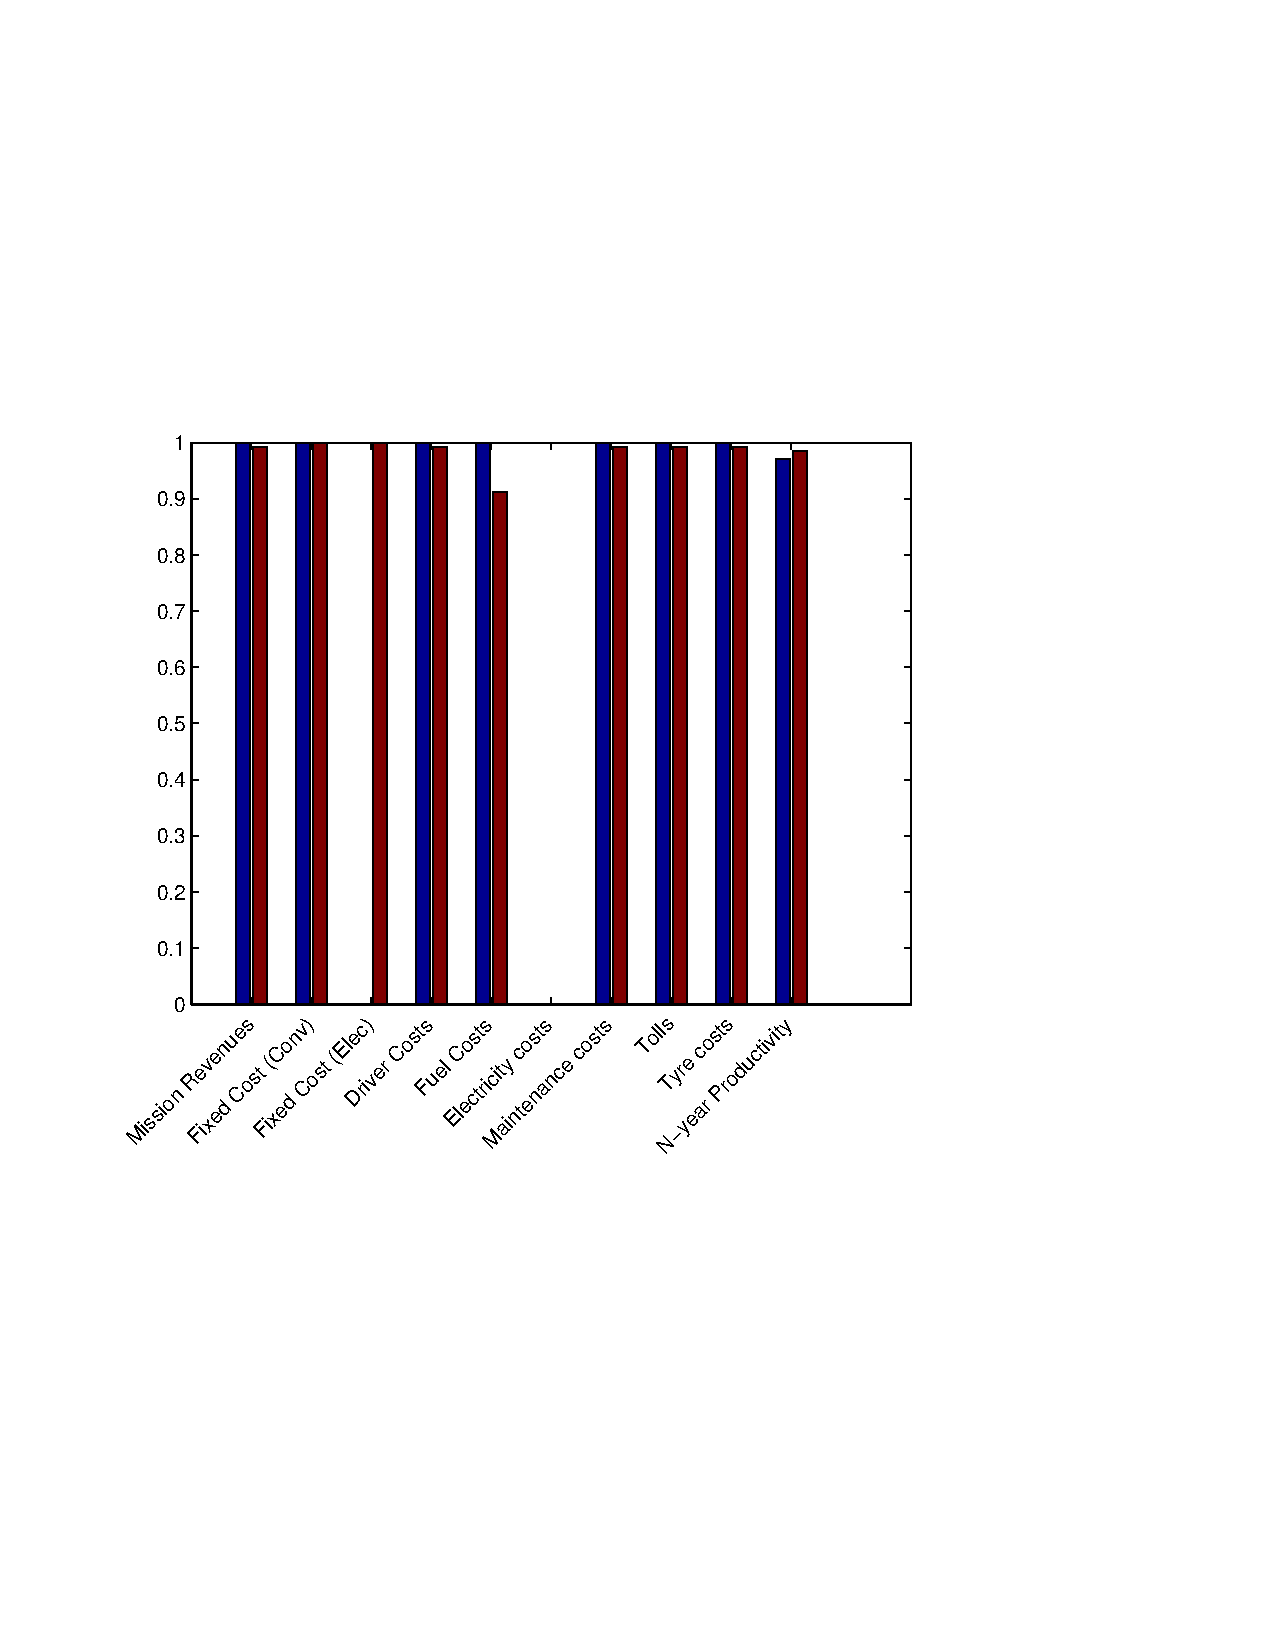
\includegraphics[width=\linewidth, clip=true, trim=45 225 135 208]{figures/OptimalCombinationResults/2015/A.pdf}
\caption{GCW=50t}
\end{subfigure}
\begin{subfigure}{.5\textwidth}
\centering
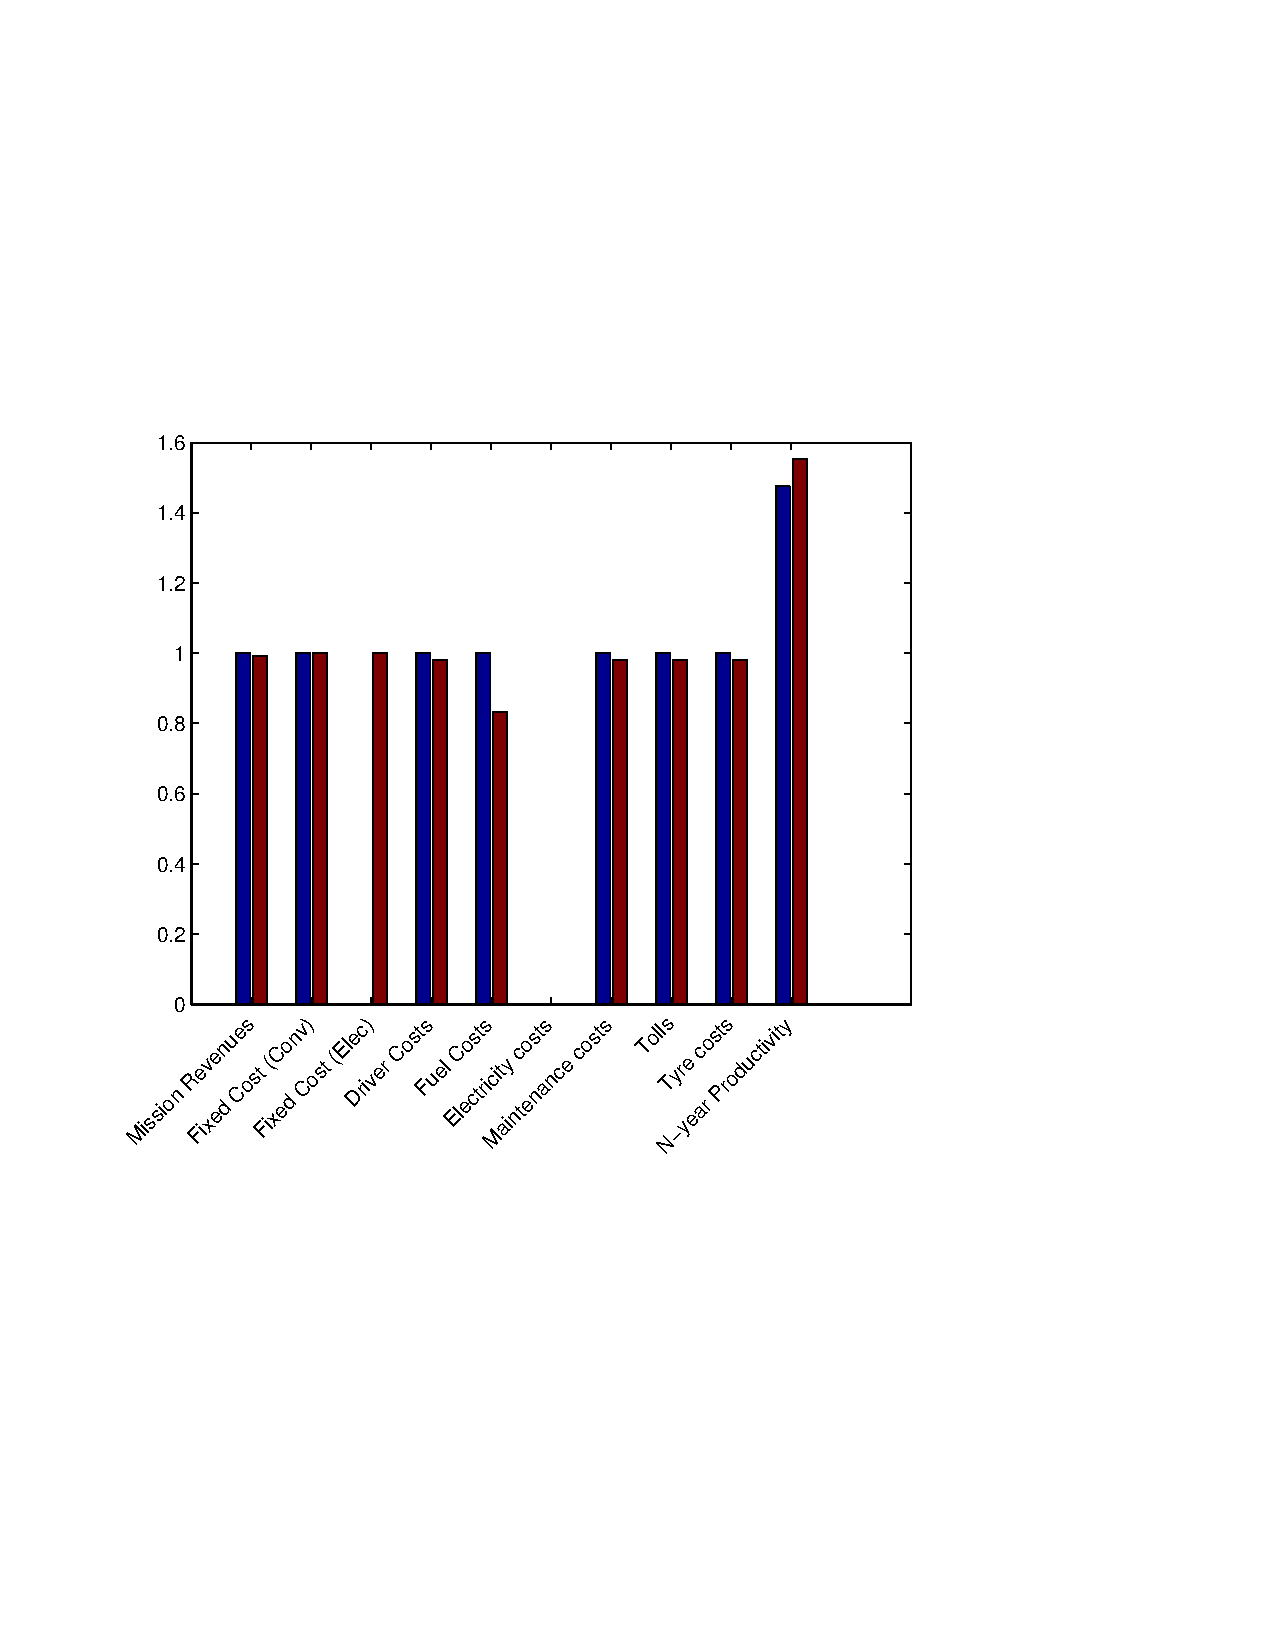
\includegraphics[width=\linewidth, clip=true, trim=45 225 135 208]{figures/OptimalCombinationResults/2020/C.pdf}
\caption{GCW=70t}
\end{subfigure}
\caption{Optimal variant compared with the conventional combination}
\label{2015AC0vsAC1}
\end{figure}

\section{Optimal Combinations for increasing GCWs}
The productivity performance of optimal configurations derived for varying GCWs in each year are observed and documented below. It can be seen in Figure \ref{prodVaryGCW2015} that optimal configurations for increasing GCWs show increased productivity. This implies that with increasing revenues, these optimal configurations bear the added advantage of reduced costs too.\\

\begin{figure}[H]
\centering
\includegraphics[width=0.5\textwidth, clip=true, trim=45 225 125 208]{figures/OptimalCombinationResults/2015/Productivity.pdf}
\caption{Variation of vehicle productivity with increasing GCW (2015)}
\label{prodVaryGCW2015}
\end{figure}

The fixed and variable costs relative to the revenues earned for each GCW are depicted in Figure \ref{fixedVariableCostVaryGCW2015}. With increased electrification, the contribution of fixed electrification costs increases for the 70t optimal configuration compared to the 60t optimal configuration, and once again reduces for the optimal configuration for 80t. The general reduction in the revenue-to-electrification cost can be attributed to reduced net payload with increasing electrification. Increased revenue-to-driver wages with increasing GCWs are also indicative of higher average speeds relative to the freight transported. The same can be said of the revenue-to-fuel costs too.\\ 

\begin{figure}[ht!]
\begin{subfigure}{.5\textwidth}
\centering
\includegraphics[width=\linewidth, clip=true, trim=45 225 65 208]{figures/OptimalCombinationResults/2015/Fixed.pdf}
\caption{Fixed costs}
\end{subfigure}
\begin{subfigure}{.5\textwidth}
\centering
\includegraphics[width=\linewidth, clip=true, trim=45 185 65 208]{figures/OptimalCombinationResults/2020/Variable.pdf}
\caption{Driver \& Fuel costs}
\end{subfigure}
\caption{Variation of fixed and variable costs with increasing GCW (2015)}
\label{fixedVariableCostVaryGCW2015}
\end{figure}

\newpage

%Similar trends are observed in the fixed costs for varying GCWs as seen in Figure \ref{fixedCostVsGCWOverYears}.\\ 

\begin{figure}[ht!]
\begin{subfigure}{.5\textwidth}
\centering
\includegraphics[width=\linewidth, clip=true, trim=45 185 65 208]{figures/OptimalCombinationResults/2015/Fixed.pdf}
\caption{Year 2015}
\end{subfigure}
\begin{subfigure}{.5\textwidth}
\centering
\includegraphics[width=\linewidth, clip=true, trim=45 185 65 208]{figures/OptimalCombinationResults/2020/Fixed.pdf}
\caption{Year 2020}
\end{subfigure}
\begin{subfigure}{.5\textwidth}
\centering
\includegraphics[width=\linewidth, clip=true, trim=45 185 65 210]{figures/OptimalCombinationResults/2025/Fixed.pdf}
\caption{Year 2025}
\end{subfigure}
\begin{subfigure}{.5\textwidth}
\centering
\includegraphics[width=\linewidth, clip=true, trim=45 185 65 210]{figures/OptimalCombinationResults/2030/Fixed.pdf}
\caption{Year 2030}
\end{subfigure}
\caption{Variation of fixed costs with increasing GCW}
\label{fixedCostVsGCWOverYears}
\end{figure}

\newpage

\begin{figure}[ht!]
\begin{subfigure}{.5\textwidth}
\centering
\includegraphics[width=\linewidth, clip=true, trim=45 185 65 208]{figures/OptimalCombinationResults/2015/Variable.pdf}
\caption{Year 2015}
\end{subfigure}
\begin{subfigure}{.5\textwidth}
\centering
\includegraphics[width=\linewidth, clip=true, trim=45 185 65 208]{figures/OptimalCombinationResults/2020/Variable.pdf}
\caption{Year 2020}
\end{subfigure}
\begin{subfigure}{.5\textwidth}
\centering
\includegraphics[width=\linewidth, clip=true, trim=45 185 65 210]{figures/OptimalCombinationResults/2025/Variable.pdf}
\caption{Year 2025}
\end{subfigure}
\begin{subfigure}{.5\textwidth}
\centering
\includegraphics[width=\linewidth, clip=true, trim=45 185 65 210]{figures/OptimalCombinationResults/2030/Variable.pdf}
\caption{Year 2030}
\end{subfigure}
\caption{Variation of driver and fuel costs with increasing GCW}
\label{variableCostVsGCWOverYears}
\end{figure}

\newpage

\section{Optimal Combinations for constant GCW over the years}

\begin{figure}[ht!]
\centering
\includegraphics[width=0.5\textwidth, clip=true, trim=45 225 125 208]{figures/OptimalCombinationResults/SingleGCW/A/Productivity.pdf}
\caption{Variation of vehicle productivity for optimal solutions for constant GCW (2015-2030)}
\label{prodConstGCWOverYears}
\end{figure}

The productivity characteristics of the optimal solutions derived for constant GCW from 2015 to 2030 is observed to increase consistently, albeit little. This can be seen in Figure \ref{prodConstGCWOverYears}. The miniscule increase in productivity can be attributed to the non-linear reduction in battery prices over the years as well as a sharper trend in fuel price rise.\\

\end{document}